\subsection{Non-Photorealistic Rendering shading styles}
As previously said, the goal of \cite{referencePaper} is to render 3D objects \textit{without any constraint} on the
choice of material or illumination, while taking into consideration the way of Geometry-based Shading technique that \textit{enhances the lighting} at each surface point. \newline
To achieve this, the authors of \cite{referencePaper} demonstrated their approach with three different \textbf{non-photorealistic shading styles}: \textit{Blinn-Phong Shading}, \textit{Cartoon shading} and \textit{Gooch} Shading. For each of those styles, they \textbf{adapted} their technique by choosing properly an \textbf{intensity mapping} function $\delta$ to be used in the reflected radiance equation.
\pagebreak
\subsubsection{Enhanced Blinn-Phong Shading implementation}
In the context of non-photorealistic rendering, it is common to make use of \textit{simple shading models} such as Blinn-Phong shading model. \newline
Geometry-based shading technique can alter surface shading to enhance surface fine-scale \textbf{geometric details} in a non-photorealistic manner. This process is performed by incorporating enhanced surface normal and surface curvature measure into Blinn-Phong.
\newline
As \textbf{intensity mapping} function \cite{referencePaper} choosed $\delta_j$ = $\rho_j$, where j $\in$ \{ a, d, s \} iterates over the components of Blinn-Phong's shading models: ambient, diffuse and specular. \newline
With this approach, using a single light, the lightning equation becomes:
\begin{equation}\label{eq:blinn1}
	L_r(x,\omega_o) = \sum_j \rho_j(\omega_o,l) \mathcal{G}_j(x,\omega_o,l) L_j(l)
\end{equation}
In this equation, l is the direction of the light source at point x, $L_j$ corresponds to the light intensity of each component, $\rho_a$ = 1, $\rho_d(l)$ = $(n'\cdot  l)$, $\rho_d(s)$ = $(n'\cdot  r)^f$; \newline
$n'(x)$ is the \textbf{enhanced surface normal}, r is the reflection direction, f is the shininess parameter and $\mathcal{G}_j(x,\omega_o,l)$ corresponds to the \textbf{Curvature-based Reflectance Scaling Function}. \newline
In particular, $\mathcal{G}_j$ is computed as:
\begin{equation}\label{eq:blinn2}
	\mathcal{G}_j(\delta, P) = \frac{\delta}{e^P (1-\delta) + \delta}\quad\mathrm{where}\quad  P_{\lambda,\alpha}(k) = pow(\lambda |k|, \alpha)
\end{equation}
In this equation, $P_{\lambda,\alpha}$ is the \textbf{curvature mapping} function; its magnitute and strength are controlled using two parameters $(\lambda,\alpha)$; $\delta$ corresponds to the previously declared \textbf{intesity mapping} function.\newline
Code-wise, I started from Blinn-Phong implementation, already present in \textbf{lecture03a} repository, and modified it following \textbf{Equations \ref{eq:blinn1}} and \textbf{\ref{eq:blinn2}} as we can see in \textbf{Code \ref{code:blinn-phong-enhanced}}, introducing all the previously listed functions. \newline
\begin{lstlisting}[language=C++, caption=Enhanced Blinn-Phong subroutine and Curvature-Based Reflectance scaling function implemented in fragment shader,label={code:blinn-phong-enhanced}]
	
	
	
	// Curvature-Based Reflectance Scaling Function
	float Lr(float curvature_value, float delta)
	{
		// We apply the curvature mapping function that uses lambda and alpha parameters to apply non-linear mapping
		float P = pow (lambda * abs(curvature_value), alpha);
		// Uses as intensity mapping function the second parameter, delta
		// This function maps intensity mapping and curvature mapping functions in the reflectance radiance equation
		// This aims to correlate the reflected lightning intensity to surface curvature
		float G = delta / ( exp(P) * ( 1 - delta ) + delta );
		return G;
	}













	// a subroutine for the Enhanced Blinn-Phong model using Shape Depiction Enhancement based on local Geometry 
	subroutine(ill_model)
	vec3 EnhancedBlinnPhong()
	{
		// Computing the mask for Unsharp Masking
		vec3 mask = vNormal - vSMNormal;
		// calculating enhanced Normal using the Unsharp Masking technique. This is defined, in the reference paper, in equation 6 of chapter 4.2.2
		vec3 eNormal = vNormal + lambda * mask;
		// normalization of the per-fragment enhanced normal 
		vec3 N_I = normalize(eNormal);
		// calculating curvature value using enhanced normal
		float curvature_value = curvature(N_I);
		// Implementing equation 12 of chapter 6.1 of the reference paper. I calculate the Curvature-Based Reflectance Scaling factor for each of the Blinn-Phong components. NOTE: Reference paper use the costant 1 as rho_a component for ambient
		float rhoA = 1;
		float G_a = Lr(curvature_value, rhoA);  
		// ambient component can be calculated at this point
		vec3 color = Ka * G_a * ambientColor;
		// normalization of the per-fragment light incidence direction
		vec3 L = normalize(lightDir.xyz);
		// Lambert coefficient
		float rhoD = max(dot(L,N_I), 0.0);
		// if the lambert coefficient is positive, then I can calculate the specular component
		if(rhoD > 0.0)
		{
			// This is the Curvature-Based Reflectance Scaling factor for the diffuse component. NOTE: Reference paper use the lambertian coefficient as rho_d for diffuse
			float G_d = Lr(curvature_value, rhoD); 
			// the view vector has been calculated in the vertex shader, already negated to have direction from the mesh to the camera
			vec3 V = normalize( vViewPosition );
			// in the Blinn-Phong model we do not use the reflection vector, but the half vector
			vec3 H = normalize(L + V);
			// we use H to calculate the specular component
			float specAngle = max(dot(H, N_I), 0.0);
			// shininess application to the specular component
			float rhoS = pow(specAngle, shininess);
			// This is the Curvature-Based Reflectance Scaling factor for the specular component. NOTE: Reference paper use the lambertian coefficient as rho_s for specular
			float G_s = Lr(curvature_value, rhoS);
			// We add diffusive and specular components to the final color using our Curvature-Based factors
			color += vec3( Kd * G_d * diffuseColor +
			Ks * G_s * specularColor);
		}
		return color;
	}

\end{lstlisting}
A Comparison between standard Blinn-Phong and Enhanced Blinn-Phong using Geometry-based shading is showed in \textbf{Figure \ref{fig:blinn_comparison}} that use two subroutines created in the project.
\pagebreak
\begin{figure}[h]
	\centering
	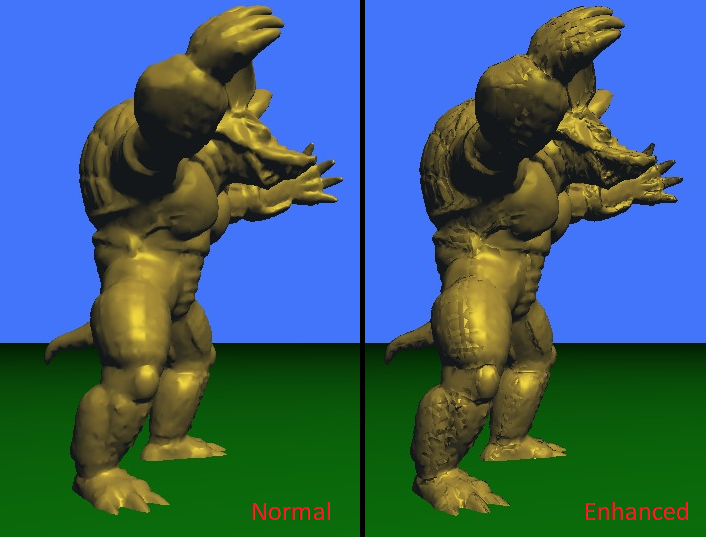
\includegraphics[width=0.8\textwidth]{Images/blinn_comparison.png}
	\caption{Comparison between standard Blinn-Phong and Enhanced Blinn-Phong using Geometry-based shading}
	\label{fig:blinn_comparison}
\end{figure}

\subsubsection{Enhanced Cartoon/Cel Shading implementation}
Cartoon shading consists of \textbf{quantizing} the amount of diffuse shading and \textbf{mapping} each discrete value to a different color. In order to apply Geometry-based shading technique, the choice of reflectance \textit{mapping function} should be consistent with this finding. To this end, \cite{referencePaper} used the following formula:
\begin{equation}\label{eq:cel1}
	\delta_d = \frac{\lfloor(0.5 + (\mathcal{Q}_L \times pow(\rho_d,r)))\rfloor}{\mathcal{Q}_L}
\end{equation}
Where $\delta_d$ corresponds to \textbf{reflected diffuse intensity} that we use in cartoon shading style, r is a \textit{power level} and it is used to enhance the intensity of color, $\mathcal{Q}_L$ is the \textit{quantization level} parameter; $\delta_a$ and $\delta_s$ are chosen in the same way as Blinn-Phong shading model.\newline
Unfortunately, \cite{referencePaper} doesn't describe how to \textbf{combine} the three components (ambient, diffuse and specular). For this reason, I choosed to introduce in the final equation two weights, for ambient and diffuse components, using the full $\delta_s$ component. \newline
The \textbf{merging equivalence} used to sum the three components togheter is:
\begin{equation}\label{eq:cel2}
	Intensity = weight_a\delta_a + weight_d\delta_d + \delta_s
\end{equation}
Code-wise, I started from implementing standard Cartoon Shading, following the paper \cite{ToonPaper}. The implementation is shown in \textbf{Code \ref{code:cel-standard}}. Then, I modify it following \textbf{Equation \ref{eq:cel1}} and \textbf{\ref{eq:cel2}} leading to the \textbf{Code \ref{code:cel-enhanced}} to obtain the final result.
\begin{lstlisting}[language=C++, caption=Standard Cartoon shading subroutine implemented in fragment shader,label={code:cel-standard}]
	// a subroutine for the Cartoon/Cel Shading model
	subroutine(ill_model)
	vec3 ToonShading(){
		// normalization of the per-fragment light incidence direction
		vec3 L = normalize(lightDir.xyz);
		// normalization of the per-fragment normal
		vec3 N = normalize(vNormal);
		// Intensity parameter used in standard toon/cel shading
		float intensity = dot(L,N);
		// Color choice based on intensity parameter
		if (intensity > 0.95)       return shinestColor;
		else if (intensity > 0.5)   return shinyColor;
		else if (intensity > 0.25)  return darkColor;
		else                        return gloomyColor;
	}
\end{lstlisting}
\begin{lstlisting}[language=C++, caption=Enhanced Cartoon shading subroutine implemented in fragment shader,label={code:cel-enhanced}]
	// a subroutine for the Enhanced Cartoon/Cel Shading model using Shape Depiction Enhancement based on local Geometry 
	subroutine(ill_model)
	vec3 EnhancedToonShading(){
		// normalization of the per-fragment light incidence direction
		vec3 L = normalize(lightDir.xyz);
		// Computing the mask for Unsharp Masking
		vec3 mask = vNormal - vSMNormal;
		// calculating enhanced Normal using the Unsharp Masking technique. This is defined, in the reference paper, in equation 6 of chapter 4.2.2
		vec3 eNormal = vNormal + lambda * mask;
		// normalization of the per-fragment enhanced normal 
		vec3 N_I = normalize(eNormal);
		// NOTE: Reference paper use the costant 1 as rho_a component for ambient
		float rhoA = 1;
		// Intensity parameter used in standard toon/cel shading, but using our enhanced normal, for the ambient compinent
		// Equation 13 of the Chapter 6.2 of the reference paper applied only to diffuse and ambient components 
		float deltaA = floor(0.5 + (Ql * pow(rhoA, r))) / Ql;
		// NOTE: Reference paper use the lambertian coefficient as rho_d for diffuse
		float rhoD = max(dot(L,N_I), 0.0);
		// Intensity parameter used in standard toon/cel shading, but using our enhanced normal, for the diffuse component
		// Equation 13 of the Chapter 6.2 of the reference paper applied only to diffuse and ambient components 
		float deltaD = floor(0.5 + (Ql * pow(rhoD, r))) / Ql;
		// Calculation of specular component, specified as in the reference paper, using the same as Phong model
		vec3 R = normalize(reflect(-L, N_I));
		vec3 V = normalize( vViewPosition );
		float specAngle = max(dot(R, V), 0.0);
		// shininess application to the specular component. NOTE: Reference paper use the lambertian coefficient as rho_s for specular
		float deltaS = pow(specAngle, shininess);
		// Composition of the final intensity to apply, then, the color choice. NOTE: In the paper is not specified how the three components are composed. This is my solution that considers only Ambient and Diffuse components, while maintaning full specular component
		float intensity = myWeightA * deltaA + myWeightD * deltaD + deltaS;
		// Color choice based on intensity parameter
		if (intensity > 0.95)       return shinestColor;
		else if (intensity > 0.5)   return shinyColor;
		else if (intensity > 0.25)  return darkColor;
		else                        return gloomyColor;
	}
\end{lstlisting}
A Comparison between standard Cartoon shading and Enhanced Cartoon using Geometry-based shading is showed in \textbf{Figure \ref{fig:cartoon_comparison}} that use two subroutines created in the project.
\begin{figure}[h]
	\centering
	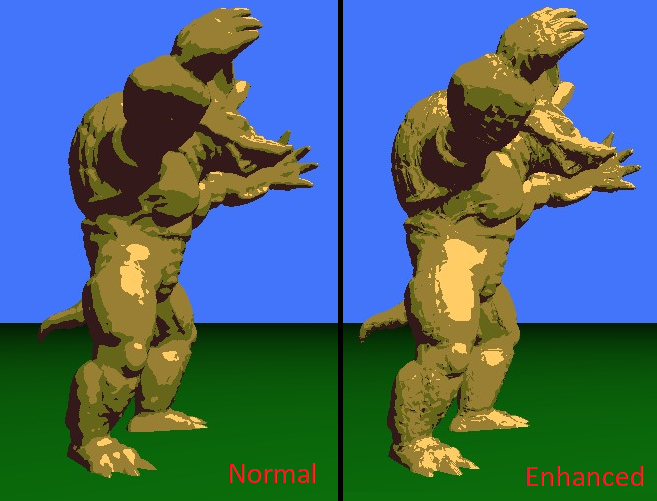
\includegraphics[width=0.8\textwidth]{Images/cartoon_comparison.png}
	\caption{Comparison between standard Cartoon shading and Enhanced Cartoon using Geometry-based shading}
	\label{fig:cartoon_comparison}
\end{figure}

\subsubsection{Enhanced Gooch Shading implementation}
Another place where a Geometry-based Shading technique is needed is when using \textbf{blending} between colors to convey the shape. The main idea in Gooch Shading is to create \textbf{cool-to-warm transition} for technical illustration. \newline
To properly scale the \textit{cool-to-warm shading}, \cite{referencePaper} use Geometry-based shading technique with Gooch shading style. The choice of the intensity mapping function is inspired by Gooch approach as following:
\begin{equation}\label{eq:gooch1}
	\delta_j = \left(\frac{1+\rho_j}{2}\right)k_{cool} + \left(1-\frac{1+\rho_j}{2}\right)k_{warm}
\end{equation}
Where j $\in$ \{a, d, s\} iterates over the ambient, diffuse, and specular component of Gooch shading model; $\rho_j$ is computed based on Blinn-Phong shading model; kcool and kwarm correspond to \textbf{cold} and \textbf{warm colors} of Gooch shading model. \newline
Unfortunately, \cite{referencePaper} doesn't describe how to \textbf{combine} the three components (ambient, diffuse and specular). For this reason, I choosed to introduce in the final equation two weights, for ambient and diffuse components, using the full $\rho_s$ component. \newline
The \textbf{merging equivalence} used to sum the three components togheter is:
\begin{equation}\label{eq:gooch2}
	Intensity = weight_a\rho_a + weight_d\rho_d + \rho_s
\end{equation}
Code-wise, I started from implementing standard Gooch Shading, following the paper \cite{GoochPaper}. The implementation is shown in \textbf{Code \ref{code:gooch-standard}}. Then, I modify it following \textbf{Equation \ref{eq:gooch1}} and \textbf{\ref{eq:gooch2}} leading to the \textbf{Code \ref{code:gooch-enhanced}} to obtain the final result.
\begin{lstlisting}[language=C++, caption=Standard Gooch shading subroutine implemented in fragment shader,label={code:gooch-standard}]
	// a subroutine for the Gooch Shading model
	subroutine(ill_model)
	vec3 GoochShading(){
		// normalization of the per-fragment light incidence direction
		vec3 L = normalize(lightDir.xyz);
		// normalization of the per-fragment normal
		vec3 N = normalize(vNormal);
		// Lambert coefficient
		float lambertian = dot(L, N);
		// weight used in standard gooch shading
		float weight = ( lambertian + 1.0 ) * 0.5;
		// Diffuse component of standard gooch shading
		vec3 kCool = min(CoolColor + DiffuseCool * SurfaceColor, 1.0);
		vec3 kWarm = min(WarmColor + DiffuseWarm * SurfaceColor, 1.0); 
		vec3 kFinal = mix(kCool, kWarm, weight);
		// Calculation of specular component
		vec3 R = normalize(reflect(-L, N));
		vec3 V = normalize( vViewPosition );
		float specAngle = max(dot(R, V), 0.0);
		// shininess application to the specular component
		float specular = pow(specAngle, shininess);
		// Final color composition of the standard gooch shading
		return vec3(kFinal + vec3(1) * specular);
	}
\end{lstlisting}
\begin{lstlisting}[language=C++, caption=Enhanced Gooch shading subroutine implemented in fragment shader,label={code:gooch-enhanced}]
	// a subroutine for the Gooch Shading model using Shape Depiction Enhancement based on local Geometry 
	subroutine(ill_model)
	vec3 EnhancedGoochShading(){
		// normalization of the per-fragment light incidence direction
		vec3 L = normalize(lightDir.xyz);
		// Computing the mask for Unsharp Masking
		vec3 mask = vNormal - vSMNormal;
		// calculating enhanced Normal using the Unsharp Masking technique. This is defined, in the reference paper, in equation 6 of chapter 4.2.2
		vec3 eNormal = vNormal + lambda * mask;
		// normalization of the per-fragment enhanced normal 
		vec3 N_I = normalize(eNormal);
		// NOTE: Reference paper use the costant 1 as rho_a component for ambient
		float rhoA = 1;
		// Equation 14 of the Chapter 6.3 of the reference paper applied only to diffuse and ambient components 
		float deltaA = (1 + rhoA) * 0.5;
		// NOTE: Reference paper use the lambertian coefficient as rho_d for diffuse
		float rhoD = max(dot(L,N_I), 0.0);
		// Equation 14 of the Chapter 6.3 of the reference paper applied only to diffuse and ambient components 
		float deltaD = (1 + rhoD) * 0.5;
		// Calculation of specular component, specified as in the reference paper, using the same as Phong model
		vec3 R = normalize(reflect(-L, N_I));
		vec3 V = normalize( vViewPosition );
		float specAngle = max(dot(R, V), 0.0);
		// shininess application to the specular component
		float rhoS = pow(specAngle, shininess);
		// Diffuse component of standard gooch shading but using our previously calculated delta as weight, for diffuse and ambient component
		vec3 kCool = min(CoolColor + DiffuseCool * SurfaceColor, 1.0);
		vec3 kWarm = min(WarmColor + DiffuseWarm * SurfaceColor, 1.0);
		vec3 kFinalA = mix(kCool,kWarm, deltaA);
		vec3 kFinalD = mix(kCool,kWarm, deltaD);
		// Composition of the final color. NOTE: In the paper is not specified how the three components are composed. This is my solution that considers only Ambient and Diffuse components, while maintaning full specular component
		return  myWeightA * kFinalA + myWeightD * kFinalD + vec3(1) * rhoS;
	}
\end{lstlisting}
A Comparison between standard Gooch shading and Enhanced Gooch using Geometry-based shading is showed in \textbf{Figure \ref{fig:gooch_comparison}} that use two subroutines created in the project.
\begin{figure}[h]
	\centering
	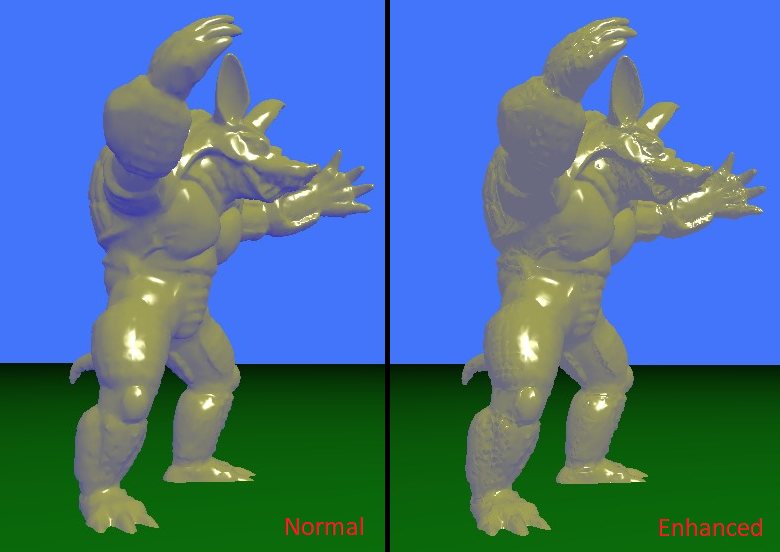
\includegraphics[width=0.8\textwidth]{Images/gooch_comparison.png}
	\caption{Comparison between standard Gooch shading and Enhanced Gooch using Geometry-based shading}
	\label{fig:gooch_comparison}
\end{figure}

